
\documentclass{article}

\usepackage[utf8]{inputenc}

\usepackage{amsmath, bm}
\usepackage{graphicx}
\usepackage{amssymb}
\usepackage{float}
\usepackage{caption}
\usepackage{subcaption}
\usepackage{hyperref}
\usepackage{tikz}
\usepackage{layout}

\usepackage[margin=1in]{geometry}
\usepackage{listings}
\usepackage{xcolor}
\usepackage{color, colortbl}
\usepackage{textgreek}
\usepackage{mathrsfs}
\usepackage{savetrees}

\usepackage{titlesec}

\titleformat{\subsubsection}
  {\normalfont\selectfont}{\thesubsubsection}{1em}{}

\usetikzlibrary{calc}
\usetikzlibrary{angles,quotes} % for pic
\usetikzlibrary{patterns,snakes}
\usetikzlibrary{arrows}
\tikzset{>=latex} % for LaTeX arrow head

\setlength{\parskip}{\baselineskip}%
\setlength{\parindent}{0pt}%
\linespread{0.9}


\definecolor{codegreen}{rgb}{0,0.6,0}
\definecolor{codegray}{rgb}{0.5,0.5,0.5}
\definecolor{codepurple}{rgb}{0.58,0,0.82}
\definecolor{backcolour}{rgb}{0.95,0.95,0.92}

\lstdefinestyle{mystyle}{
    backgroundcolor=\color{backcolour},   
    commentstyle=\color{codegreen},
    keywordstyle=\color{magenta},
    numberstyle=\tiny\color{codegray},
    stringstyle=\color{codepurple},
    basicstyle=\ttfamily\footnotesize,
    breakatwhitespace=false,         
    breaklines=true,                 
    captionpos=b,                    
    keepspaces=true,                 
    numbers=left,                    
    numbersep=5pt,                  
    showspaces=false,                
    showstringspaces=false,
    showtabs=false,                  
    tabsize=2
}

\lstset{style=mystyle}


\begin{document}

\title{}
\author{lwp26}
\date{November 2024}
\maketitle 

\iffalse
\begin{abstract}
    \centering
    LOg bAs
\end{abstract}
\fi

%-----------------------------------------------------------------------------------------
\section{Introduction}
%-----------------------------------------------------------------------------------------

\subsection{Objectives}

\subsection{Setup}

\begin{figure}[H]
    \centering
    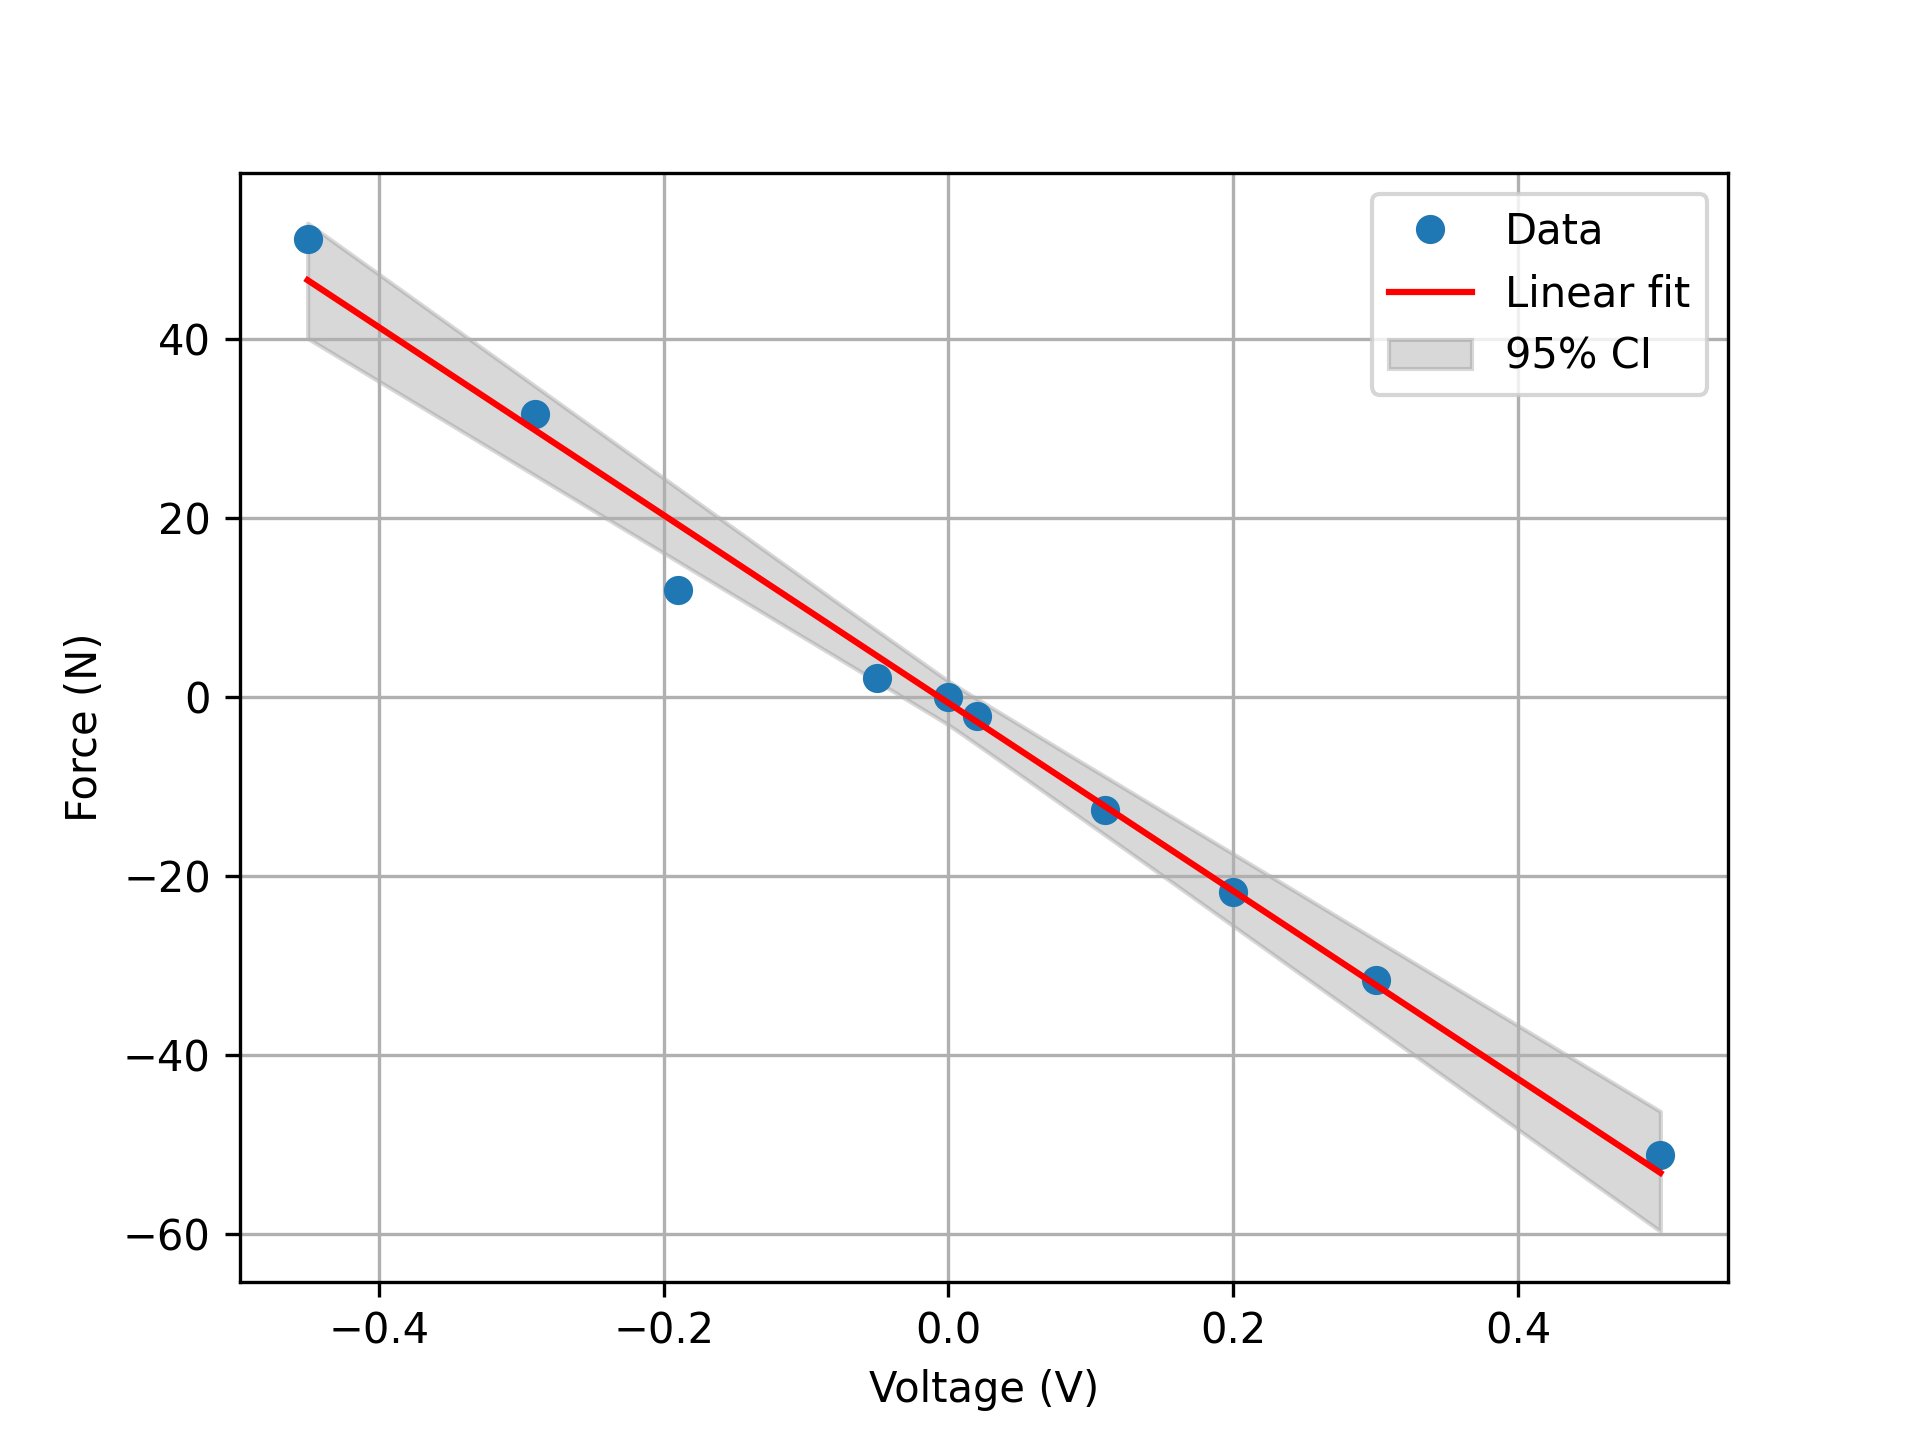
\includegraphics[width=0.8\textwidth]{Calibration/linearity.png}
    \caption{Loss coefficient for various operating Mach and Reynolds numbers.}
    \label{fig:force_linearity}
\end{figure}

\section{Discussion}

\section{Appendix}

\begin{thebibliography}{9}


  \bibitem{handout}
  J. V. Taylor
  \emph{Turbine Cascade Aerodynamics Handout}
  University of Cambridge,
  October 2024.

  \bibitem{losses}
  J. D. Denton (1993).
  \emph{Loss Mechanisms in Turbomachines}
  May, 1993 

  \bibitem{fluidmech}
  S. L. Dixon
  \emph{Fluid Mechanics, Thermodynamics of Turbomachinery, FOURTH EDITION}
  1998

  \bibitem{separation}
  John M. Russell
  \emph{LENGTH AND BURSTING OF SEPARATION BUBBLES: A PHYSICAL INTERPRETATION}
  1979
\end{thebibliography}

\end{document}